\subsection{Приведение интеграла}
Метод Монте-Карло основан на аппроксимации интеграла с помощью среднего значения функции, вычисленного в случайных точках. Для удобства генерации таких точек и обеспечения их равномерного распределения, область интегрирования отображается на единичный куб \([0,1]^n\). Это преобразование позволяет использовать стандартные генераторы случайных чисел, равномерно распределенных в диапазоне \([0,1]\).

Так рассмотрим область \([a, A] \times [b, B] \supset D\), мы хотим задать отображение, причем следующее верно:
\begin{align}
	\varphi \colon R^2 \to R^2 \\
	\varphi \colon [0, 1]^2 \mapsto [a, A] \times [b, B]
\end{align}
Задать такое преобразование можно как аффинное. А раз преобразование аффинное, то оно является и диффеоморфизмом. А значит мы можем использовать формулу замены переменных.
\begin{align}
	\int\limits_{D=\varphi(D')}f(x)dx = \int\limits_{D'}f(\varphi(t))|\varphi'(t)|dt.
\end{align}
При том \(|\varphi'(t)| = |J_t\varphi|\) --- якобиан преобразования \(\varphi\).

Более конкретно, задаем замену:
\begin{align}
	\begin{cases}
		x = a + (A - a) \xi \\
		y = b + (B - b) \eta
	\end{cases},
\end{align}
тогда якобиан равняется:
\begin{align}
	|\varphi'| = \begin{vmatrix}
		             x'_\xi & x'_\eta \\
		             y'_\xi & y'_\eta
	             \end{vmatrix} = \begin{vmatrix}
		                             A - a & 0     \\
		                             0     & B - b
	                             \end{vmatrix} = (A - a) (B - b),
\end{align}
а интеграл принимает вид:
\begin{align}\label{eq:ab-iint}
	I = (A - a)(B - b)\iint\limits_{D'}f(\varphi(t))dt
\end{align}
Для заданного примера:
\begin{align}
	\begin{cases}
		x = 2 + 4 \xi \\
		y = \frac{4}{3} + \frac{32}{3} \eta
	\end{cases}
\end{align}
\begin{align}
	I = \frac{128}{9}\iint\limits_{D'}(16 + 24\xi + 32\eta)d\xi d\eta,
\end{align}
где
\begin{align}
	D'\colon \begin{cases}
		         \xi < 1      \\
		         4\eta-3\xi<1 \\
		         (2+4\xi)(4+32\eta)>24
	         \end{cases}
\end{align}

\begin{figure}[h]
	\begin{subfigure}{.5\textwidth}
		\centering
		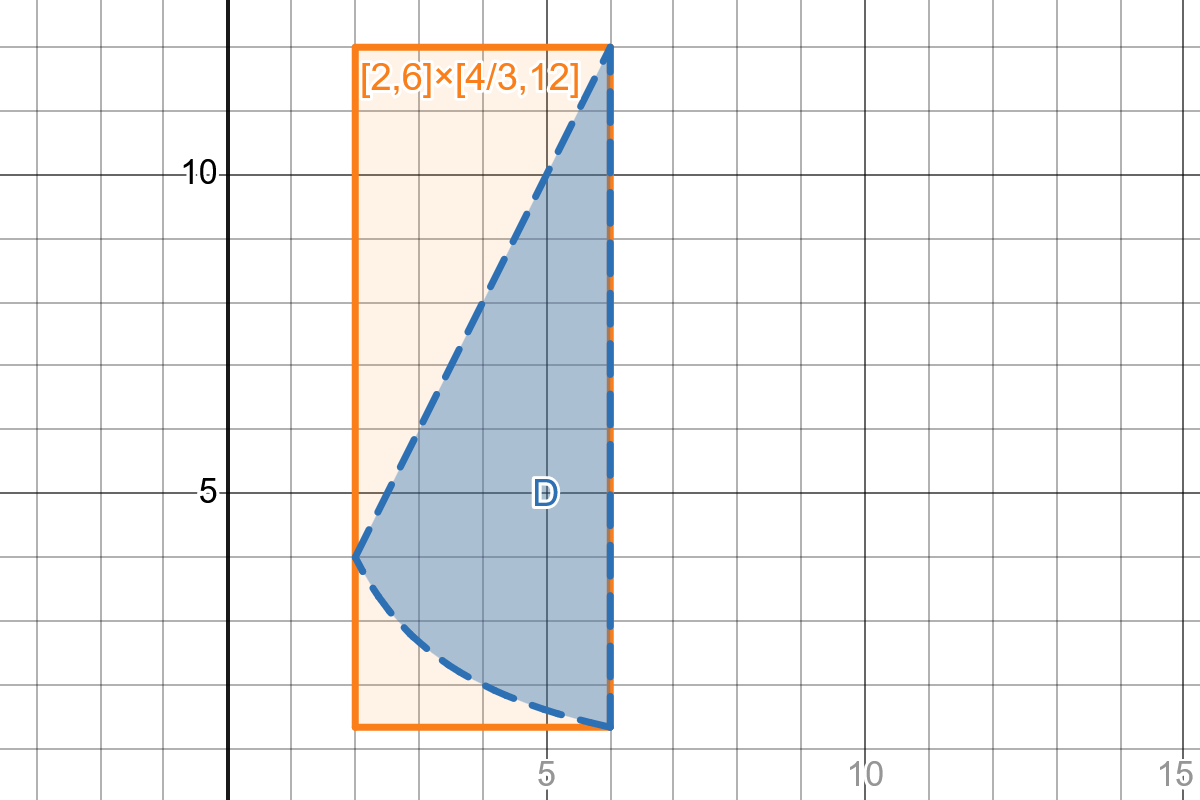
\includegraphics[width=.8\linewidth]{D-D1.png}
		\caption{Область \(D\)}
	\end{subfigure}
	\begin{subfigure}{.5\textwidth}
		\centering
		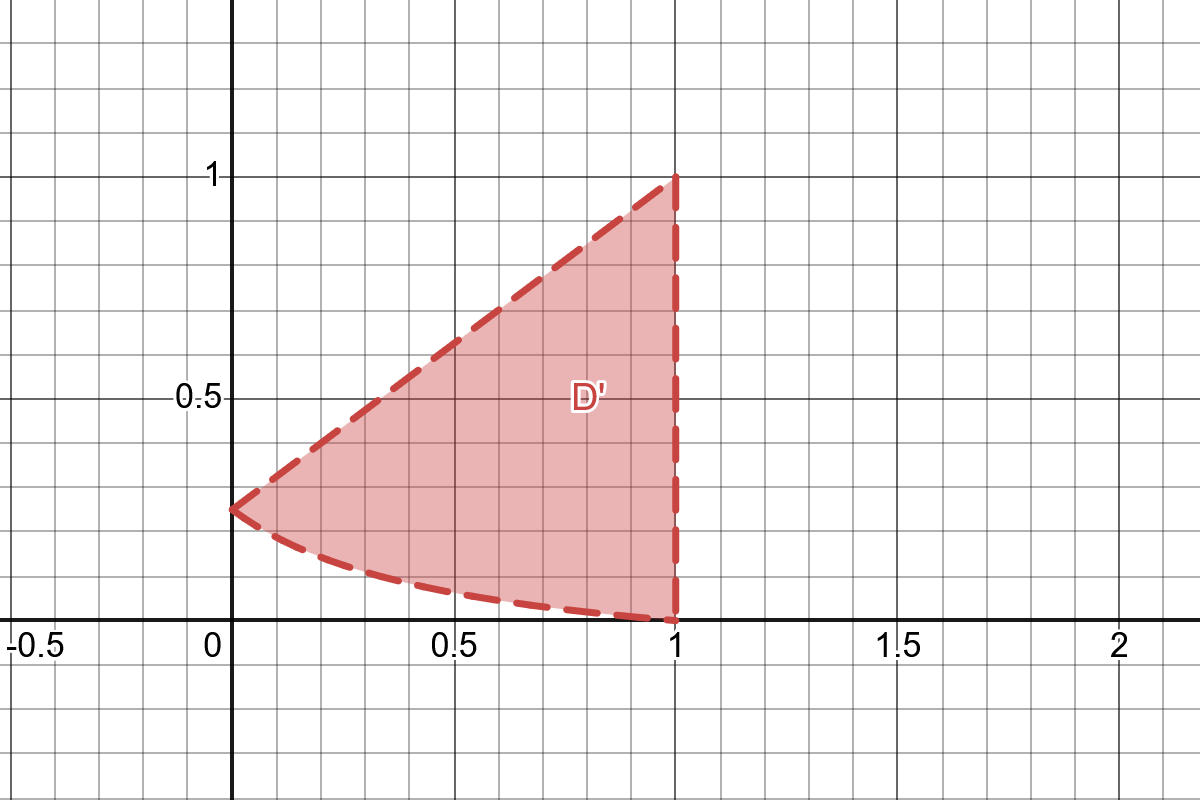
\includegraphics[width=.8\linewidth]{D1.png}
		\caption{Область \(D'\)}
	\end{subfigure}
\end{figure}
